\section{Experiments}
\label{sec:exp}

\begin{table*}
  \begin{centering}
    \scalebox{0.75}{
      \begin{tabular}{|c|c|c|c|c|c|}
        \hline 
        \textbf{Dataset} & \textbf{Domain} & \textbf{\#Class} &
        \textbf{\#Training Samples} & \textbf{\#Samples/Class} & \textbf{Settings}\tabularnewline
        \hline 
        ITG & FAQ chatbot & 228 & 3938 * 0.7 & 12 & 3-fold\tabularnewline
        \hline 
        Amazon-670k & Product review & 250 & 2658 * 0.7 & 8 & 3-fold\tabularnewline
        \hline 
        HWU64 & Intent detection & 64 & [320, 640, 960, 1280, 1920, 3200] & [5, 10, 15, 20, 30, 50] & data sampling\tabularnewline
        \hline 
        CLINC150 & Intent detection & 150 & [750, 1500, 2250, 3000, 4500, 7500] & [5, 10, 15, 20, 30, 50] & data sampling\tabularnewline
        \hline 
        BANKING77 & Intent detection & 77 & [385, 770, 1155, 1540, 2310, 3850] & [5, 10, 15, 20, 30, 50] & data sampling\tabularnewline
        \hline 
        FRAMES & Intent detection with NER & 21 & [208, 408, 984] & [10, 20, 50] & data sampling\tabularnewline
        \hline
        ATIS & Intent detection with NER & 21 & [168, 303, 544] & [10, 20, 50] & data sampling\tabularnewline
        \hline
      \end{tabular}
    }
    \par
  \end{centering}
  \caption{Statistics for all datasets and few shot settings.}

  \label{tbe:dataset statistic}
\end{table*}

\subsection{Datasets}
Our experiments aim to study the short text classification in the low-resource environment popular in the task-specific conversational chatbot application.
The datasets adopted in our experiments, showed in Table \ref{tbe:dataset statistic} \footnote{All settings of six public datasets would be released to github soon.}, typically contain comparatively large number of class labels, ranging from several dozens to hundreds, and each class label is associated with a handful of labeled queries with each query being usually one sentence. 

\emph{ITG}, is a proprietary FAQ dataset from real-world
chatbot project, which is composed of question and answer pairs about online
English teaching. It contains 3,938 sample questions for 228 class labels, and
each class label corresponds to a unique answer.

\emph{Amazon-670K}, is a customer product review dataset for
text classification task from the extreme classification repository. The
complete dataset contains 670,091 class labels, 285,176 training samples and
150,875 testing samples \cite{bhatia2016extreme}. As each sample may
correspond to multiple class labels, we keep only the first one. We further
filter out the class labels that only associated to training samples within the amount of 5 to 15 to mimic the few-shot chatbot scenario. From them, we sample 250 class
labels as well as their training samples to form a subset with 2658 samples.

\emph{HWU64}, is an intent detection dataset designed for
home robot scenario \cite{liu2019benchmarking}. It aims at the specific task
of capturing the intent for different user requests to home robot and
finding the corresponding answer. The raw dataset contains 25,716 data points
for 64 class labels through crowdsourcing.

\emph{CLINC150}, is a dataset designed for task-oriented
systems with 23,700 queries that are short and unstructured for 150 intents,
in the same style made by real users through crowdsourcing
\cite{larson2019evaluation}.

\emph{BANKING77}, is an intent detection dataset for bank
customer services. The raw dataset contains 13,084 data points for 77 class
labels \cite{casanueva2020efficient}.

\emph{FRAMES}, is a collection of multi-domain dialogues dealing with
hotel bookings. The raw data is consists of 1369 human-human
dialogues with slot filling information. There are 30,522 utterances in total for 21 intents and 49 slots \cite{asri2017frames}.

\emph{ATIS}, is a popular dataset for intent detection of flight reservations with slot filling\cite{tur2010left}. The raw data's training, development and test sets contain 4,478, 500 and 893 utterances, respectively. There are 120 slot labels and 21 intent types for the training set.

Regarding the first two datasets, we conduct 3-fold cross validation experiments that treat 70 percent as training, 15 percent as validation and testing respectively, and report the averaged testing results. 
Regarding the last five datasets, we use a sampling method similar to that from \cite{casanueva2020efficient} yet in a more sophisticated few-shot settings. 
We fix a test data for each one, and examine their performances using 5, 10, 15, 20, 30, or 50 samples per class label respectively for training. 
This is important, as in practice a task-specific chatbot usually starts with merely a handful of labeled data available in the early stage.
Besides, in the active learning framework, building an effective auxiliary system with limited resource is also quite important to help developers label new data more efficiently.

\subsection{Baselines}
Our baselines comprise of \emph{four} styles of systems. 

The first one, \emph{non-pretrained model based classification system}, which consists of a typical CNN based TextCNN \cite{kim2014convolutional}, and a label-embedding based LEAM \cite{wang2018joint}. 
Regarding TextCNN, the input is from RoBERTa tokenization, and the kernels are set as 1, 2, 3, 4, 5. 
Regarding LEAM, a literal class label is required, which is available only in HWU64, CLINC150, BANKING77. 
Thus, for other two datasets, we have to use its class number instead. 
Empirically, a non-pretrained model based system are not performing as well as a pretrained models based in many NLP tasks.
Our listing these non-pretrained model based systems here is serving a comprehensive performance comparison on our datasets.

The second one, \emph{pretrained model based classification system}, which consists of BERT \cite{devlin2018bert}, RoBERTa \cite{liu2019roberta}, and ALBERT \cite{lan2019albert} based. 
These pretrained models are practically proven to achieve outstanding performances in classification task and other NLP tasks.

The third one, \emph{pretrained model based similarity model}. 
As RoBERTa is empirically found more effective than other pretrained models in the short text classification task in our experiments, we choose RoBERTa-large based implementation.
In inference, we use an elastic search to find a set of potential candidate labels for the similarity model, to guarantee a reasonable running time.

The fourth one, \emph{pretrained model based joint text classification and NER model}. 
We choose the work from \cite{chen2019bert} as our baseline system, which utilizes a strong RoBERTa-large model to jointly train two losses.

All pretrained model baselines are fine-tuned on our datasets.
Especially, the similarity model baseline and all similarity layers in SFCs use extra Quora dataset \cite{iyer2017first} \footnote{which contains 404,290 potential duplicate question pairs} to enhance system performance. 
This is also one of merits in SFC, as it support adopting out-of-domain data in comparison to a classification based model.

Our SFC implementations include three 2-stage SFCs using task 1 and 2 with ablation in Table \ref{tbe:table2}; one joint SFC trained on all three tasks in Table \ref{tbe:table2}; one joint SFC with an additional fourth NER task in Table \ref{tbe:addtional ner experiments}. 

\subsection{Result Analysis}
We report the F1 score \footnote{In the multi-class and multi-label case, this
is the average of the F1 score of each class with weighting depending on the
numbers in each class.} as the main evaluation measure for all experiments in
Table \ref{tbe:table2} and Table \ref{tbe:addtional ner experiments}.

\subsubsection*{Multi-task and joint training} 
\begin{table}
  \begin{centering}
    \scalebox{0.65}{
      \begin{tabular}{|c|ccc|ccc|}
        \hline
        \multicolumn{1}{|c|}{\multirow{2}*{\textbf{Models}} }& \multicolumn{3}{c|}{\textbf{FRAMES}}& \multicolumn{3}{c|}{\textbf{ATIS}}\tabularnewline
        \cline{2-7}
        \multicolumn{1}{|c|}{} & $\textbf{10}$ & $\textbf{20}$ & $\textbf{50}$
        & $\textbf{10}$ & $\textbf{20}$ & $\textbf{50}$\tabularnewline
        \hline
        RoBERTa-large & \multirow{2}*{${0.3456}$} & \multirow{2}*{${0.4043}$} & \multirow{2}*{${0.4262}$} & \multirow{2}*{${0.9349}$} & \multirow{2}*{${0.9757}$} & \multirow{2}*{${0.9800}$}\tabularnewline
        (classification) & & & & & & \tabularnewline
        \hline
        RoBERTa-large & \multirow{3}*{${0.3520}$} & \multirow{3}*{${0.4088}$} & \multirow{3}*{${0.4353}$} & \multirow{3}*{${0.9560}$} & \multirow{3}*{${0.9706}$} & \multirow{3}*{$\textbf{0.9832}$}\tabularnewline
        (classification & & & & & & \tabularnewline
        w/ NER) & & & & & & \tabularnewline
        \hline
        Joint SFC & \multirow{2}*{${0.3843}$} &
        \multirow{2}*{${0.4130}$} & \multirow{2}*{${0.4390}$} &
        \multirow{2}*{${0.9618}$} & \multirow{2}*{${0.9761}$} & 
        \multirow{2}*{${0.9825}$}\tabularnewline
        (w/o NER) & & & & & & \tabularnewline
        \hline
        Joint SFC & \multirow{2}*{$\textbf{0.3925}$} &
        \multirow{2}*{$\textbf{0.4420}$} & \multirow{2}*{$\textbf{0.4456}$} &
        \multirow{2}*{$\textbf{0.9639}$} & \multirow{2}*{$\textbf{0.9784}$} & 
        \multirow{2}*{${0.9826}$}\tabularnewline
        (w/ NER) & & & & & & \tabularnewline
        \hline
      \end{tabular}
    }
  \end{centering}

  \caption{
    F1 scores for joint sentence classification and NER training. 
    We iterate various sample number per intent and test on original test set.
  }
  \label{tbe:addtional ner experiments}
\end{table}

\begin{table}
  \begin{centering}
    \scalebox{0.85}{
      \begin{tabular}{|c|c|c|c|}
        \hline
        F1 score & 2-stage SFC & joint SFC & Gap \tabularnewline
        \hline
        top-1 accuracy & \textbf{81.50} & 81.07 & -0.47 \tabularnewline
        top-5 accuracy & 94.01 & \textbf{94.30} & +0.29 \tabularnewline
        \hline
      \end{tabular}
    }
    \par
  \end{centering}
  \caption{The average classification accuracy in percentage in stage 1 on the first five datasets.}
  \label{tbe:top1_5_accuracy}
\end{table}

Comparing with training 2-stage SFC with multi-task Table \ref{tbe:table2}, training with only task 1, namely the sentence pair similarity model, degrades by 0.8 percentage point on average, and training with only task 2, namely the top-K based classification task, degrades by 0.45 percentage point on average. 
These degradation indicates multi-task training in 2-stage SFC is helpful for the system performance. Besides, task 2 plays a relatively more important role in multi-task learning, and this aligns with their optimal weight settings.

Joint SFC consistently outperforms 2-stage SFC with multi-task training on 5 diverse datasets by 0.95 percentage point on average. 
Though a joint model structure may bring extra complexity to the system, it does alleviate the error propagation from the first stage and improves the final performance.

In following analysis, we will focus on the comparison between joint SFC and the other baseline models.

\subsubsection*{Fusion of classification and similarity models} 
%We compare joint SFC with classification, similarity and NER joint model based baselines respectively.

\begin{table}
  \begin{centering}
    \scalebox{0.58}{
      \begin{tabular}{|c|c|c|c|c|c|c|}
        \hline 
        \multicolumn{1}{|c|}{\multirow{2}*{Dataset}}&\multicolumn{1}{c|}{\multirow{2}*{Model}}& $K=3$ & $K=5$ & $K=10$ & $K=15$ & $K=20$\tabularnewline
        \multicolumn{1}{|c|}{} & \multicolumn{1}{c|}{} & $P=20$ & $P=10$ & $P=5$ & $P=4$ & $P=3$\tabularnewline
        \hline
        \multicolumn{1}{|c|}{\multirow{2}*{ITG}}& 2-stage SFC & $0.8034$ & $0.8124$ & $0.8008$ & $0.7967$ & $0.7934$\tabularnewline
        \cline{2-7}
        \multicolumn{1}{|c|}{} & joint SFC & $0.7986$ & $0.8114$ & $0.8010$ & $0.7972$ & $0.7918$\tabularnewline
        \hline
        \multicolumn{1}{|c|}{\multirow{2}*{Amazon-670k}}& 2-stage SFC & $0.7278$ & $0.7364$ & $0.7366$ & $0.7328$ & $0.7204$\tabularnewline
        \cline{2-7}
        \multicolumn{1}{|c|}{} & joint SFC & $0.7334$ & $0.7445$ & $0.7516$ & $0.7344$ & $0.7373$\tabularnewline
        \hline
      \end{tabular}
      \par
    }
  \end{centering}
  \caption{
    The performances of SFC from different settings of hyperparameters, $K$ denoting the candidate class number from stage 1,
    $P$ denoting the number of sampled sentence pair in stage 2. 
  }
  \label{tbe:table3}
\end{table}

Regarding the classification models, joint SFC outperforms RoBERTa-large based, the strongest among all baselines, by 2.04 percentage points on average F1 score over 5 datasets. 
Especially, ALBERT.xxlarge based is rather unstable in this short sentence task. 
Thus, we run multiple times with different settings and report the best ones here. 
Comparatively, RoBERTa based is the most stable and has the best performance almost all experiment settings.

Regarding the similarity model, as analyzed above, we only choose the RoBERTa-large based implementation as our baseline. 
Joint SFC achieves more improvement of 7.09 percentage points on average F1 score. 
This is also understandable, since RoBERTa-large based similarity model does not and also can not train towards the task specific goal.

The above analysis illustrates that suitable fusing these two kinds of models can take their advantages.

\subsubsection*{Joint SFC improves stage 1?}
We explore the quality of predicted candidate labels in stage 1 from 2-stage SFC and joint SFC respectively. 
We should note that 2-stage SFC does not optimize the stage 1 model, namely a RoBERTa based classification model.

From Table \ref{tbe:top1_5_accuracy}, the joint training does not improve the top-1 classification accuracy in stage 1, yet it improves the top-5 accuracy.
The reason is that, a classification model inherently optimizes the objective loss, 0-1 error of top-1 here; the sentence pair similarity model in joint SFC poses more positive effect in optimizing the candidate labels.

\subsubsection*{Supportive of extra NER task}
Many previous work shows joint training with a NER task improves the intent classification task as well, observed again in our baselines and SFCs in Table \ref{tbe:addtional ner experiments}.
Our SFC systems set the weight of the fourth NER task as 0.25 throughout this part. 

We can see that our joint SFC without a NER task still outperforms RoBERTa baseline with a NER task by 0.86 percentage points on average. 
This indicates that the fusion of classification and similarity models can even works better than fusing with additional NER information under few-shot chatbot scenario. 

Moreover, the adding NER task to joint SFC further achieves improvement of 1.66 percentage points over RoBERTa baseline with a NER task. 
Especially on FRAMES dataset, which is a much more difficult task in comparison with ATIS based on performance of all systems on it, our joint SFC with a NER task achieves a bigger improvement of 2.8 percentage points on average. 

\subsubsection*{Different training sample size} 
We analyze the overall improvement trend of joint SFC under various few-shot settings, and show results in Fig. \ref{fig:trend}.

Our main focus is on studying chatbot construction in real world applications, where each class has only a small number of example sentences.
The experimental results for the 3 diverse intent detection datasets (ClINC150, BANKING77, HWU64) under few-shot settings, 5 to 50 samples per class, indicate that our proposed joint SFC can achieve average 2.47 percentage points improvement over one of the most powerful baseline models, which is RoBERTa-large classification model. 
Moreover, the improvement in F1 score becomes more and more prominent with the decrease of data sample number per class.

\begin{figure}[t]
  \begin{centering}
    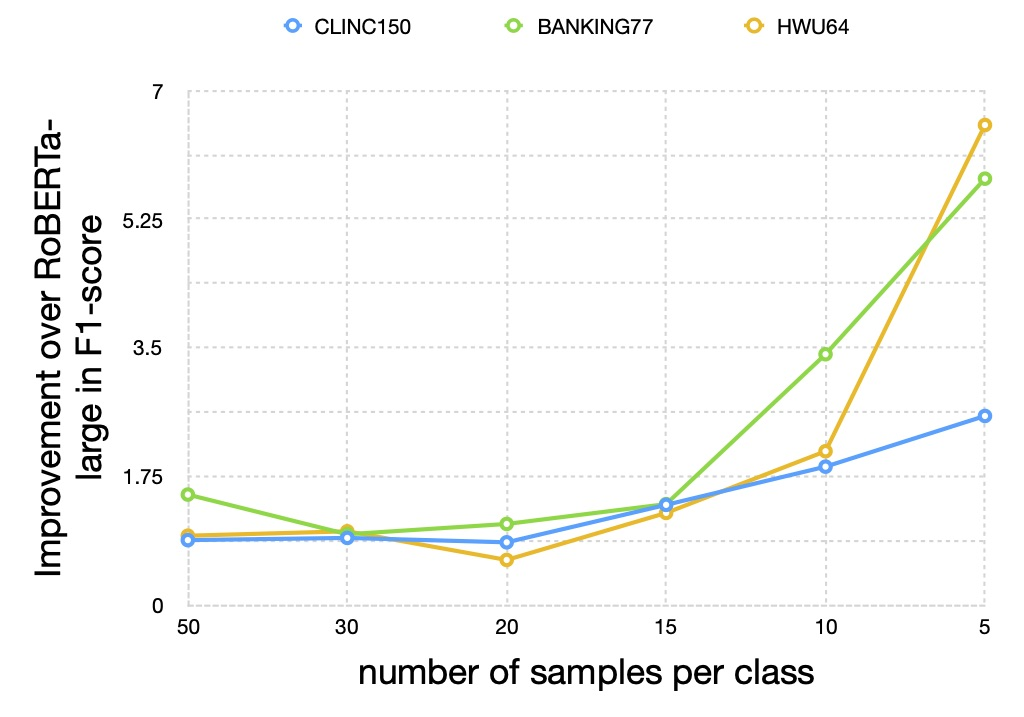
\includegraphics[scale=0.2]{picture/improvement_trend.jpg} 
    \par
  \end{centering}
  \caption{
    Improvements from joint SFC over RoBERTa based classification with different training size.
  }
  \label{fig:trend}
\end{figure}

Especially, in the most extreme setting with only 5 training samples per class, joint SFC achieves 4.97 percentage points improvements on average over RoBERTa-large classification model. 
Joint SFC is a better choice applied into the early stage of building a task-specific chatbot system, since label data is extremely scarce.

Furthermore, joint SFC also achieves average 2.04 percentage points improvement over RoBERTa-large classification model on all the data settings. 
However, the improvement is still more prominent when the data is scarce, which makes SFC an excellent model for low-resource chatbot scenario.

\subsection{Settings of hyperparameters} 
In Table \ref{tbe:table3}, we explore the influence from hyperparameters on ITG and Amazon-670K datasets. 
We control the total number of sampled sentence pairs to about 50 to 60, and obtain about five combinations of hyperparameters. 

We find that the best setting of hyperparameters is different with different datasets. 
The class label number of ITG and Amazon-670k are similar in our experiments, around 250. 
However the number of data points in ITG is approximately 2 times as many as that in Amazon-670k.
Therefore, the setting of $K=5$ and $P=10$ is good enough for ITG since most of the classes contains over 10 data points. 
However, in Amazon-670k, the data per each class is scarce, and, we may need more candidate classes to sample enough effective sentence pairs for the stage 2 training of SFC. 
Thus, the setting of $K=10$ and $P=5$ becomes a good choice. 

However, despite the effect on evaluation performance brought by different settings of hyperparameters, joint SFC still steadily outperforms two-stage SFC by 0.41 percent points in overall average F1 score on ITG and Amazon-670k datasets.

For the experiments in Table \ref{tbe:table2}, we empirically set the hyperparameter to be $K=5$ and $P=10$ for all SFC variants. 

\subsection{Other settings}
We fine-tune all SFC systems with the maximum sequence length of 128, learning rate of 1.5e-5 for RoBERTa-large pretrained model and 5e-4 for task-specific layer with a linear decay, and use Adam optimizer.

In two-stage SFC, in equ. \ref{eq:two-stage_SFC_loss} the weights of two tasks are set as $\alpha_S=0.125$ and $\alpha_K=0.875$ in our setting. 
In joint SFC, in equ. \ref{eq:joint_SFC_loss}, the weights of three tasks are set as $\alpha_S=0.25$, $\alpha_K=0.25$ and $\alpha_C=0.5$. 
Overall, the task weights are less sensitive in joint SFC than in two-stage SFC.

As for the training time, in our settings, our joint SFC model needs about 14 hours to reach convergence using a single Nvidia RTX8000 GPU. 
In comparison, the classification baseline model needs about 5 hours and the similarity baseline model needs about 12 hours.

